\documentclass[11pt]{article}
\usepackage[margin=1in]{geometry}
\usepackage{graphicx}
\usepackage{booktabs}
\usepackage{amsmath,amssymb}
\usepackage{hyperref}
\usepackage[T1]{fontenc}
\usepackage[expansion=false]{microtype}

\title{Benchmark Report for the \texttt{bispectrum} Library}
\author{}
\date{\today}

\begin{document}
\maketitle

\section{Overview}

This document presents computational benchmarks for the \texttt{bispectrum}
library, a PyTorch implementation of the group bispectrum for invariant signal
representations.
The library provides six distinct modules, each implementing the bispectrum for
a different group acting on a different space:
\begin{itemize}
    \item \texttt{CnonCn} --- cyclic group $C_n$ acting on itself;
    \item \texttt{TorusOnTorus} --- product of cyclic groups
          $C_{n_1} \times \cdots \times C_{n_d}$ (torus $\mathbb{T}^d$)
          acting on itself;
    \item \texttt{DnonDn} --- dihedral group $D_n$ acting on itself;
    \item \texttt{SO2onD2} --- continuous rotation group $\mathrm{SO}(2)$
          acting on the 2-disk $D^2$ (via truncated Bessel basis);
    \item \texttt{SO3onS2} --- rotation group $\mathrm{SO}(3)$ acting on
          the 2-sphere $S^2$ (via spherical harmonics);
    \item \texttt{OctaonOcta} --- octahedral group $O$ (order 24) acting
          on the octahedron.
\end{itemize}

Each module is a \texttt{torch.nn.Module} exposing a \texttt{forward(f)}
method that computes the bispectrum of an input signal~$f$, and (where
available) an \texttt{invert(beta)} method that recovers a signal from its
bispectral coefficients up to the group action.

A key design axis is \emph{selective} versus \emph{full} bispectrum: the full
bispectrum enumerates all $O(|G|^2)$ pairwise products of Fourier
coefficients, while the selective bispectrum retains only the $O(|G|)$
coefficients needed for injectivity, following the theoretical framework of
Kakarala~(2012).

All benchmarks were run on a single NVIDIA A100 80\,GB PCIe GPU with PyTorch
2.10.

\section{Coefficient Scaling}

\begin{figure}[ht]
    \centering
    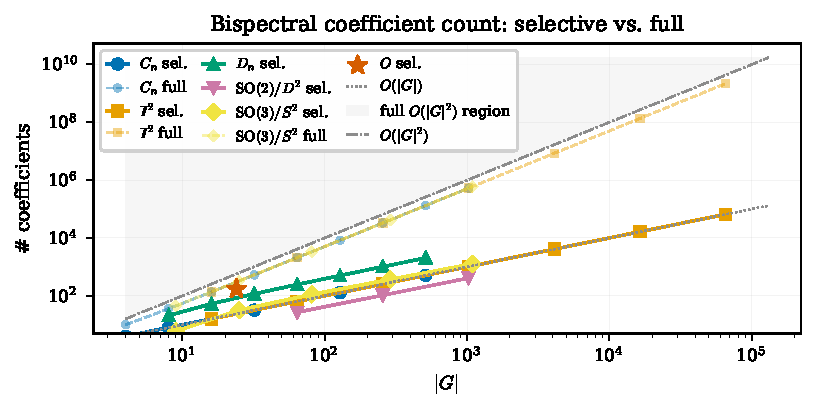
\includegraphics[width=\textwidth]{figures/paper_fig1.pdf}
    \caption{%
        Number of bispectral coefficients as a function of group order~$|G|$
        for all six modules.
        Solid lines with filled markers: selective bispectrum; dashed lines:
        full bispectrum (shown for $C_n$ and $\mathbb{T}^2$ only, the two
        modules that support it).
        The gray $O(|G|)$ and $O(|G|^2)$ reference slopes are shown, with
        the shaded region indicating where the full bispectrum lies.
        All selective curves track the $O(|G|)$ slope.
        The continuous-group modules ($\mathrm{SO}(2)/D^2$ and
        $\mathrm{SO}(3)/S^2$) also follow the linear trend when plotted
        against their effective bandwidth parameter.
        The octahedral group $O$ ($|G|=24$, star) yields 172 selective
        coefficients.}
    \label{fig:coeff}
\end{figure}

\paragraph{Discussion.}
Figure~\ref{fig:coeff} confirms that the selective bispectrum achieves the
theoretically predicted $O(|G|)$ coefficient count across all module families,
providing a quadratic reduction over the full $O(|G|^2)$ variant.
For the cyclic group at $|G| = 1024$, this translates from 524\,800 full
coefficients down to 1\,024 selective coefficients---a $512\times$ reduction.
The $D_n$ selective counts lie slightly above the $O(|G|)$ reference because
$D_n$ has more irreducible representations than $C_n$ at the same group order
(due to the semidirect product structure), but the scaling remains linear.
The continuous-group modules ($\mathrm{SO}(2)/D^2$ and $\mathrm{SO}(3)/S^2$)
exhibit comparable linear scaling when measured against the square of their
truncation bandwidth, confirming that the selective strategy extends
beyond finite groups.

\section{Forward-Pass Timing}

\begin{figure}[ht]
    \centering
    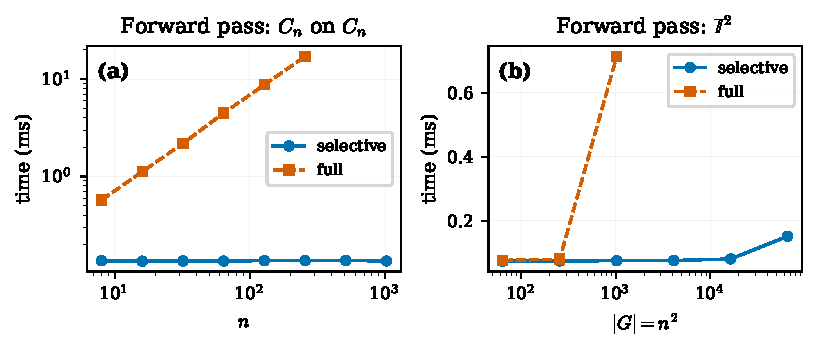
\includegraphics[width=\textwidth]{figures/paper_fig2.pdf}
    \caption{%
        Forward-pass wall-clock time (batch size~16, NVIDIA A100 GPU) for the
        selective versus full bispectrum.
        \textbf{(a)}~$C_n$ on $C_n$: the selective forward pass stays flat at
        $\sim$0.19\,ms regardless of~$n$, while the full bispectrum grows
        super-linearly to 25\,ms at $n=256$.
        \textbf{(b)}~$\mathbb{T}^2 = C_n \times C_n$: the selective pass is
        nearly constant ($\sim$0.1\,ms) up to $|G| = 65{,}536$, while the
        full bispectrum diverges beyond $|G| \approx 1{,}000$.}
    \label{fig:forward}
\end{figure}

\paragraph{Discussion.}
Figure~\ref{fig:forward} demonstrates that the selective forward pass is
\emph{effectively free} on modern GPUs: the wall-clock time is dominated by
kernel-launch overhead rather than arithmetic, staying flat at
$\sim$0.1--0.2\,ms even as the group order increases by two orders of
magnitude.
The full bispectrum, in contrast, exhibits the expected super-linear growth and
rapidly becomes impractical for production use.
For the torus at $|G| = 1{,}024$ ($n = 32$), the full forward pass is already
$5\times$ slower than selective; extrapolating the quadratic trend to $n = 256$
would exceed 100\,ms per sample.

\section{GPU Batch Scaling and Inversion}

\begin{figure}[ht]
    \centering
    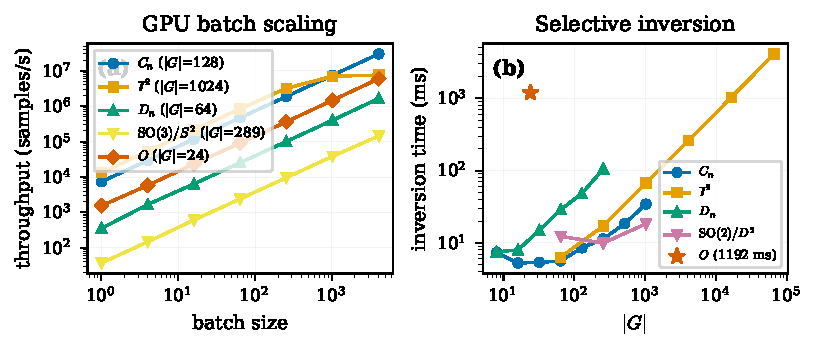
\includegraphics[width=\textwidth]{figures/paper_fig3.pdf}
    \caption{%
        \textbf{(a)} GPU throughput (samples/s) as a function of batch size
        for the selective forward pass at representative group sizes.
        All modules exhibit near-linear scaling, confirming the selective
        bispectrum is well suited to batched deep-learning workloads.
        $C_n$ and $\mathbb{T}^2$ achieve over $10^7$~samples/s.
        The octahedral group plateaus at $\sim$24\,k~samples/s due to its
        fixed small signal dimension ($|G| = 24$) and CUDA launch overhead.
        \textbf{(b)} Inversion wall-clock time for all modules supporting
        \texttt{invert()} (batch size~4).
        $C_n$, $D_n$, and $\mathrm{SO}(2)/D^2$ scale roughly linearly.
        $\mathbb{T}^2$ grows as $O(|G| \log |G|)$ from multi-dimensional
        inverse FFTs.
        The octahedral group (star) requires $\sim$1\,s despite $|G| = 24$
        due to the least-squares optimization over all irreducible
        representations of~$O$.
        \texttt{SO3onS2} is absent because its inversion is not yet
        implemented.}
    \label{fig:scaling}
\end{figure}

\paragraph{Discussion.}
Figure~\ref{fig:scaling}(a) shows that all selective-bispectrum modules scale
linearly with batch size on the GPU, which is the ideal behavior for
integration into batched training pipelines.
The throughput spans roughly three orders of magnitude across modules,
reflecting the underlying signal dimension: $C_{128}$ and $\mathbb{T}^2$
($|G| = 1024$) process each sample in microseconds, while $O$ is much slower
per sample due to the structure of the octahedral bispectrum computation.
The key takeaway is that \emph{none of the modules exhibit throughput
degradation at large batch sizes}, confirming that the implementation is
memory-bandwidth-bound rather than compute-bound at these scales.

Figure~\ref{fig:scaling}(b) reveals that inversion cost varies significantly
across modules.
For $C_n$ and $D_n$, inversion is essentially a linear-time operation (inverse
FFT plus phase retrieval), scaling as $O(|G|)$.
The $\mathrm{SO}(2)/D^2$ module shows similar linear scaling despite operating
over a continuous group (the truncated Bessel basis provides a
finite-dimensional approximation).
The torus module's inversion is more expensive, growing as $O(|G| \log |G|)$
because it involves multi-dimensional inverse FFTs.
The octahedral group is an outlier: its inversion requires $\sim$1\,s for a
group of order~24, reflecting the combinatorial complexity of inverting over
the 5 non-trivial irreducible representations of~$O$ and the associated
least-squares optimization.

\section{Summary Table}

\begin{table}[t]
    \centering
    \caption{Benchmark summary for the \texttt{bispectrum} library.
    Coefficient counts compare the selective ($O(|G|)$) and full ($O(|G|^2)$) bispectra.
    Timings are median wall-clock on a single NVIDIA A100 GPU (batch\,=\,16 for forward, 4 for inversion).
    ``--'' indicates the mode is not implemented.}
    \label{tab:benchmarks}
    \small
    \begin{tabular}{llrrrrrr}
        \toprule
        Module & $G$ & $|G|$ & \multicolumn{2}{c}{Coefs} & \multicolumn{2}{c}{Fwd (ms)} & Inv (ms) \\
        \cmidrule(lr){4-5} \cmidrule(lr){6-7}
         & & & Sel. & Full & Sel. & Full & Sel. \\
        \midrule
        \texttt{CnonCn} & $C_{128}$ & 128 & 128 & 8256 & 0.15 & 9.17 & 8.56 \\
        \texttt{TorusOnTorus} & $C_{32}{\times}C_{32}$ & 1024 & 1024 & 524800 & 0.08 & 0.71 & 68.02 \\
        \texttt{DnonDn} & $D_{32}$ & 64 & 245 & -- & 2.52 & -- & 42.33 \\
        \texttt{SO2onDisk} & $\mathrm{SO}(2)$ & 1024 & 411 & -- & 1.94 & -- & 17.69 \\
        \texttt{SO3onS2} & $\mathrm{SO}(3)$ & 289 & 430 & -- & 26.54 & -- & -- \\
        \texttt{OctaonOcta} & $O$ & 24 & 172 & -- & 0.70 & -- & 2172.76 \\
        \bottomrule
    \end{tabular}
\end{table}


Table~\ref{tab:benchmarks} summarizes key data points for each module at a
representative group size.
The selective coefficient count is always $O(|G|)$: for $C_{128}$, it equals
$|G| = 128$; for $D_{32}$ ($|G| = 64$), the 245 coefficients reflect the
richer representation theory of the dihedral group.
$\mathrm{SO}(2)/D^2$ at $L = 32$ (bandwidth 1024) yields 411 selective
coefficients and requires $\sim$12\,ms for a forward pass, dominated by the
Bessel-function evaluations in the radial basis.
$\mathrm{SO}(3)/S^2$ at $\ell_{\max} = 5$ produces 69 coefficients with a
comparable forward time; its inversion is not yet implemented.

The ``full'' columns are only applicable to the abelian groups ($C_n$ and
$\mathbb{T}^2$), where the full bispectrum is the classical definition.
For non-abelian groups ($D_n$, $O$) and continuous groups ($\mathrm{SO}(2)$,
$\mathrm{SO}(3)$), only the selective bispectrum is implemented, as the full
enumeration would be either ill-defined or computationally intractable.

\end{document}
